\subsection{Concepts d'agriculture de précision}
La croissance exponentielle de la population~\cite{wiki:popu_mondiale}
au cours des dernières décennies et par conséquent le besoin de nourrir
tout le monde, ne laisse pas d'autres choix
si ce n'est celui d'optimiser l'agriculture.
Cependant le concept d'optimisation de l'agriculture peut 
paraître assez flou et général.
Une définition assez intuitive d'une agriculture optimisée
peut être d'essayer d'obtenir
les récoltes les plus bénéfiques en ayant une consommation minimum d'énergie
et d'intrants (eau, engrais\dots) en tenant compte de facteurs à la fois
agronomiques, environnementaux et économiques~\cite{wiki:agri_prec}.

C'est précisemment ce que vise l'agriculture de précision.
Globalement, on dira que \enquote{l'agriculture de précision désigne
l'ensemble des techniques culturales basées sur l'utilisation
des nouvelles technologies de mesure et de traitement de l'information
spatialisée}~\cite{jullien2005agriculture}.

À ce jour les coûts engendrés par les installations technologiques
nécessaires pour utiliser les systèmes d'agriculture de précision
mais l'investissement est souvent rentabilisé à long, surtout 
dans le cas de grandes parcelles.
En effet, cette nouvelle forme d'agriculture ne permet pas seulement
d'être bénéfique pour les sols et nappes phréatiques,
elle engendre également une diminution des dépenses de l'agriculteur
par une consommation moins importante d'engrais et d'eau.
À cet diminution d'utilisation d'engrais s'associe une réduction
d'émissions de particules néfastes pour
environnement telles que des nitrates, phosphates
et pesticides~\cite{emission_agri_particules}.
Ce dernier point semble d'autant plus important dans le contexte
écologique actuel où le respect de l'environnement est nécessaire
d'un point vue légal mais aussi moral.

\begin{figure}
  \begin{center}
    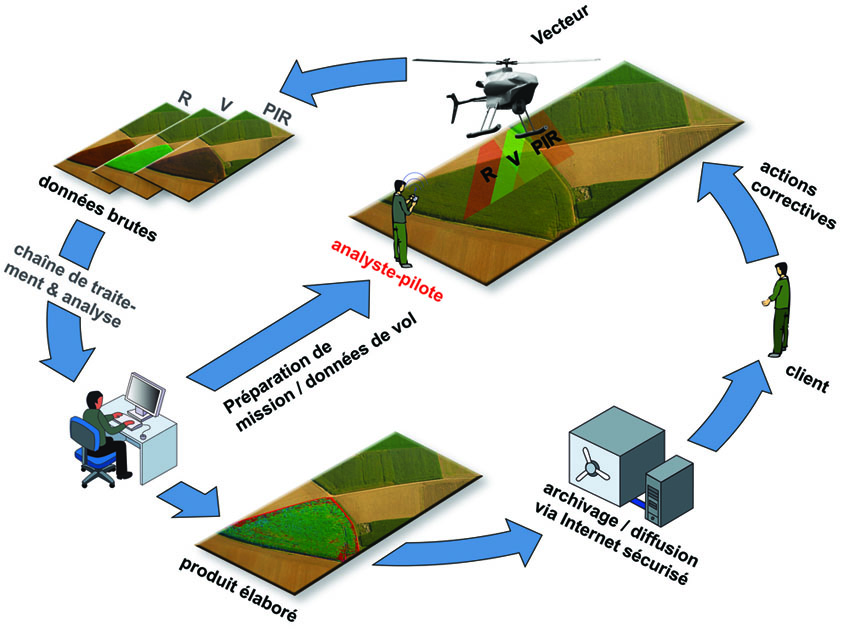
\includegraphics[scale=0.42]{./img/agridrone.jpeg}
  \end{center}
  \caption{Représentation d'une application d'agriculture de 
  précision~\cite{vegedrones}.
  On retrouve un système d'acquisition d'images sur drones ainsi
  qu'une analyse rétroactive des données récupérées.}
\end{figure}